\chapter{Bayesian Optimization}
This chapter will introduce Bayesian optimization. However, we start with an introduction to the optimization
framework in general. 

\section{Optimization methodology}
Given a cost/objective function $f: \mathcal{X} \rightarrow \mathbb{R}$, where the domain
$\mathcal{X}$ could be a subset of $\mathbb{R}^n$,
optimization is a methodology which seeks to find an optimal point, $x^*$, and value
$f^* = f(x)$, given as
\begin{align}\label{OPT}
    x^* \in \arg\min_{x \in \mathcal{X}} f(x) \hspace{1cm} f^* = \min_{x \in \mathcal{X}} f(x) = f(x^*).
\end{align}
Note that the above formulation is a minimization problem, which is equivalent to a
maximization problem maximizing $-f(\cdot)$. Throughout this thesis, we choose to only work
with a minimization problem. 
Solving this problem is intractable except for rare cases e.g. if $f$ is 
convex and analytically directly solvable or the domain of $f$ is very limited. Hm

\begin{testexample}[Direct solution method]
    The unconstrained linear least squares, $$\min_{x\in \mathbb{R}^n} f(x) := ||Ax-b||_2^2$$
    where $A \in \mathbb{R}^{m\times n}$ and $b \in \mathbb{R}^m$, is a convex problem,
    i.e. finding $x^*$ such that $\nabla f(x^*) = 0$ is equivalent to finding the solution
    to the problem. Assuming $A^TA$ is invertable, linear least squares can be solved
    directly by the normal equations, 
    $$\nabla f(x) = 2A^TAx + 2b^TA = 0 \hspace{0.5cm} \Leftrightarrow \hspace{0.5cm} x^* = (A^TA)^{-1} A^Tb$$
\end{testexample}

Most optimization problems are non-convex with multiple local minima. And even if the gradient is
given analytically the solution is found among a potentially infinitely large 
set of stationary points ($\nabla f(x) = 0$) and boundary points - this might be tedious or impossible.
When the problem is not directly solvable, mathematical optimization takes an indirect methodology: 
Design a sequence of experiments that reveal information of the objective function. This information 
can hopefully lead us to the solution of \eqref{OPT}. This general way of sequentially solving 
is presented in the book Bayesian Optimization by Roman Garnett \cite{bayesoptbook} and 
presented here as Algorithm \ref{algOPT}. 
W
\begin{algorithm}
\caption{Sequencial Optimization \cite{bayesoptbook} }\label{algOPT}
\begin{algorithmic}
\State \textbf{Input:} Initial dataset $\mathcal{D}$  \Comment{can be empty}
\While{Temination is not reached}
    \State $x \gets \text{policy}(\mathcal{D})$ \Comment{select next observation location}
    \State $y \gets \text{observe}(x)$ \Comment{observe objective function at chosen location}
    \State $\mathcal{D} \gets \mathcal{D} \cup \{(x,y)\} $ \Comment{update dataset}
\EndWhile
\State $\textbf{return: } \mathcal{D}$
\end{algorithmic}
\end{algorithm}

Given data points in the optimization landscape\footnote{"Optimization landscape" defined as the joint set of points in the domain and the objective function
evaluated in the points, i.e. $\{(x,f(x))\in \mathcal{X} \times \mathbb{R}| x \in \mathcal{X}\}$} 
a policy selects a point $x \in \mathcal{X}$ where we make our next observation. Policies can be deterministic or probibalitic, e.g. 
grid search and random search are examples of policies. The next observation provides us a $y$ value, which combined with $x$ is included to the 
available data $\mathcal{D}$. Finaly, a stopping criterion decides whether to continue or terminate. 

<example of random search is half as efficient as BO>


\begin{testexample}[Grid search]
    In grid search values along each dimention in $\mathcal{X}$ is seleced and combined with each
    other, which thereby defines a grid in the parameter space. All points are ordered and systematicly
    selected. In the content of algorhtim \ref{algOPT} we define the grid search policy as 
    $$\text{policy}_{GS}(\mathcal{D}) = x_{|\mathcal{D}|+1}$$
    assuming $x_1,x_2, \dots, x_{n}$ are the ordered grid points and the size of the obtained 
    data is $|\mathcal{D}|$. 
\end{testexample}
\begin{testexample}[Random search]
    In random search a uniform distribtuion is layed over the domain space $\mathcal{X}$ and a random point
    is selected from the distribtuion. 
    $$\text{policy}_{RS}(\mathcal{D}) = x, \hspace{0.5cm} x \sim p(\mathcal{X})$$
    Note that grid search and random search are policies which completely 
    ignores the available data. This is a shame and we can do better. 
\end{testexample}

\begin{testexample}[Gradient descent]
    Gradient descent is the most simple gradient-based optimization approach. The gradient of a continuous 
    function points in the most ascending direction from the location where it is evaluated.
    In the minimization task, \eqref{OPT}, we can iteratively use the opposite gradient direction, i.e. the most 
    descenting directiong. This yields the policy:
    $$\text{policy}_{GD}(\mathcal{D}) = x_n - \eta \nabla f(x_n)$$
    where we for a brief moment modify $y$ to be a vector, since the observation model 
    is given as:
    $$\text{observe}_{GD}(x) = [f(x), \nabla f(x)]$$
\end{testexample}

\begin{testexample}[Surrogate-based optimization]
    <SVR> <Radial Basis function> <Polynomal model/respons surface>
    In surrogate-based optimization all available data is fitted by a cheap-to-evaluate approximation
    to the objective function - this approximation is called a \textit{surrogate} model. Examples
    of surrogate models could be a neural network or a random forest. The next point is 
    chosen as the point where the surrogate model is minimized. 
    $$\text{policy}_{sur}(\mathcal{D}) = \min_x \hat f(x)$$
    where $\hat f(x) \approx f(x)$ for $x$ close to the data $\mathcal{D}$. And we hope the approximation
    holds for $x$ far away from the the data. \textbf{}
\end{testexample}

\subsection{When to use Bayesian optmization}
What if $f(x)$ took serval days to evaluate. What if $f(x)$ is noisy? what if discrete points? 
<more here>

% \begin{figure}[h]
%     \centering
%     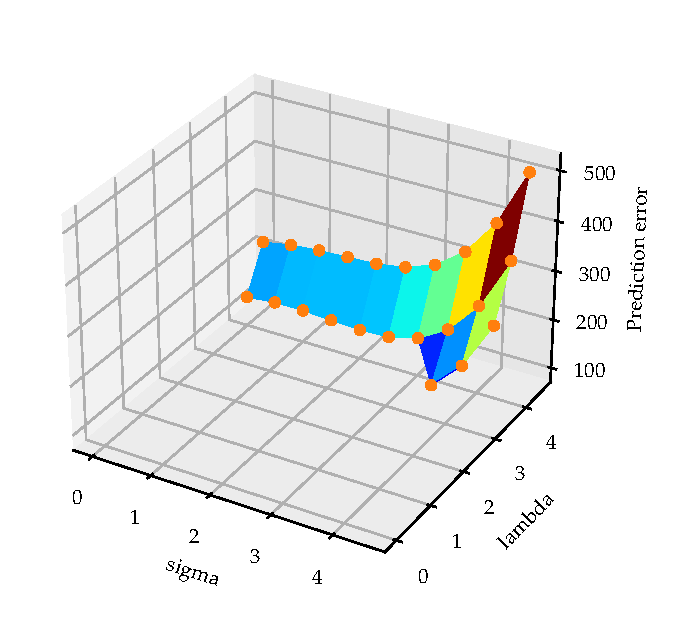
\includegraphics[width=0.9\textwidth]{Pictures/BO_vs_Grid2.eps}
%     \caption{Hyper parameter tuning of a model $M(\lambda, \sigma)$, 
%     35 evaluation in grid search vs 39 evaluations using Bayesian optimization}
%     \label{optimhist}
% \end{figure}
\begin{tcolorbox}[
    sharp corners,
    boxrule=0mm,
    enhanced,
    borderline west={4pt}{0pt}{gray},
    colframe=drGray,
    colback=drGray,
    coltitle=black,
]
{\large \textbf{Example: Bayesian Optimization}}\\
    Bayesian optimization is a \textit{probabilistic} surrogate-based optimization
    methodology. Here a cheap probabilistic regression model $p(y|x)$ is fitted to the
    the observations $\mathcal{D}$ and oppose to (deterministic) surrogate-based
    optimization, it is not possible right away to find the minima in the cheap
    surrogate model; first, we need to interpret the meaning of minima in a probabilistic
    regression model. This interpretation is done through a so-called acquisition
    function (more about this later). The policy is as following,
    $$\text{policy}_{BO}(\mathcal{D}) = \max_x AQ(p(y|x))$$
\end{tcolorbox}
\begin{figure}[H]%
    \centering
    {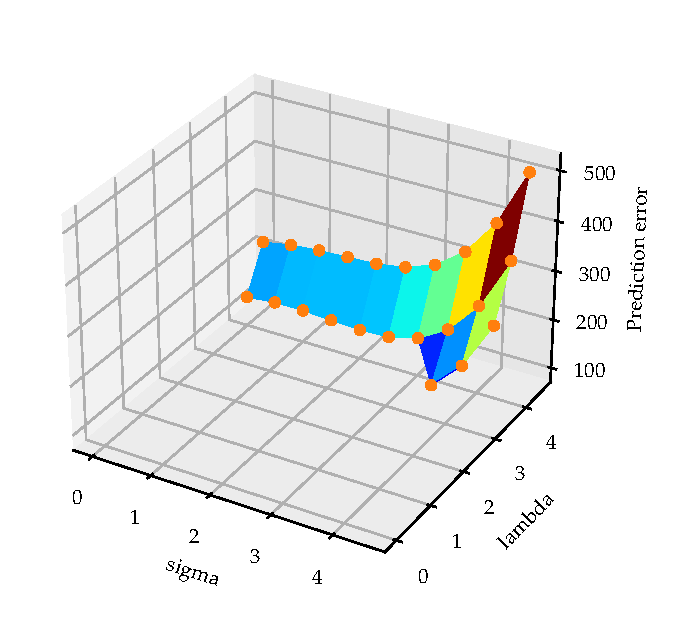
\includegraphics[width=0.46\textwidth]{Pictures/BO_vs_Grid2.eps} }%
    \qquad
   {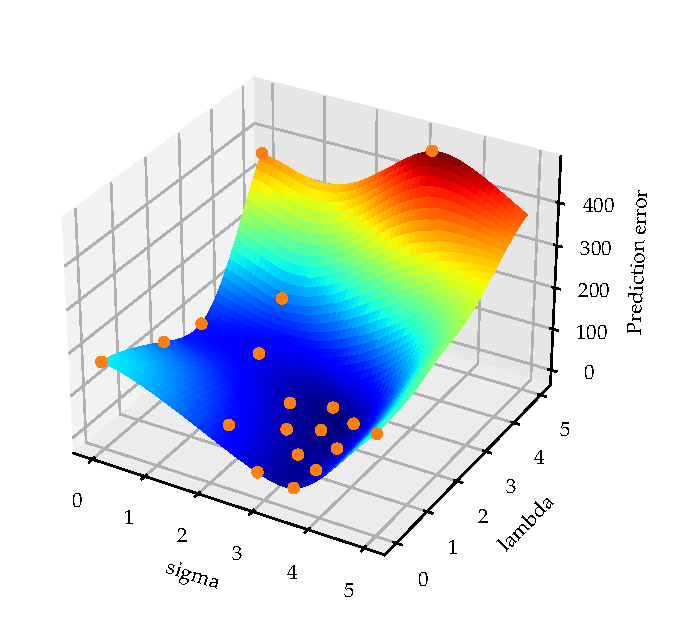
\includegraphics[width=0.46\textwidth]{Pictures/BO_vs_Grid1.eps} }%
    \caption{Hyper parameter tuning of a model $M(\lambda, \sigma)$, 
    23 evaluation in grid search vs 23 evaluations using Bayesian optimization}%
    \label{fig:example}%
\end{figure}


additionally, Bayesian Optimization allow for observation noise, 

\subsection{Observation model}\label{ObsModel}
Many optimization algorithms assume \textit{exact} evaluations of the objective function. However, this assumption
is often wrong especially for objective functions with real-life experiments, imperfect simulations, human interaction 
where measurement noise is a well known. The observation model is typically noisy and described as
$$y = f(x)+\epsilon$$ where $\epsilon$ is the measurement error, this is
typically assumed to be Gaussian with zero mean and a variance
$\sigma^2$ (which could depend on $x$ in a heterostodatic setting) and implies a Gaussian observation model, 
$$p(y|x,f(x),\sigma) = \mathcal{N}(y;f(x),\sigma^2)$$ 

% (note from now on we define $\phi := f(x)$ in order to avoid confusion and a extra set of paranteses)
% $$p(y|x,\phi,\sigma) = \mathcal{N}(y;\phi,\sigma^2)$$ 
we can extend this model to deal with noiseless observations as well, simply by setting $\sigma = 0$ and let the
model colaps into a Direct delta distribution, 
$$p(y|x, f(x)) = \mathcal{\delta}(y-f(x))$$
i.e. all probability mass for $y$ is on the value $f(x)$ giving the observation sample $y = f(x)$





\section{Bayesian Optimization}
<Cope with inacuracies> i.e. allows for stochastic objective function. 
<Uncertainty measure with prediction based on simple and clear prior 
assumptions about the characteristic about the objective function. >
<Provides an adequate termination condition for the opt. process>. 

<kilde 151. Bayes Opt is assumes superior to other global optimization tequnies 
with limited budget>


Whereas traditional regression workflow is the following: From data, fit model parameters, make predictions using the parameters. 
The Bayesian framework allows us to skip the dependency of a single set of parameters and instead use all sets of parameters 
by treating the set of parameters as a random quantity, $\theta$. What is of interest is the predictive posterior distribution,  
\begin{align}\label{Predictive2}
    p(y|x, \mathcal{D})
\end{align}
% Before bringing the parameters/unknown quantities into play, we can ask: What quantities can we play
% with? This question is answered in two different ways in Gaussian process regression and Bayesian
% Neural network regression.

Bayesian optimization is essentially two steps: First, a probabilistic surrogate-model is fitted
to the available data $\mathcal{D}$ giving the predictive distribution \eqref{Predictive2}. Second,
the next sample point is chosen according to a so-called acquisition function, which in a sense
balance out the well-known concept, exploitation and exploration. Where exploitation will be chooing
the next point according to its expected improvement and exploration will be choosing the next point
in a region of high uncertainty and thereby help lower the overall uncertainty. We will first look at
the acquisition function used in this thesis, which is also the most commonly used: E   xpected improvement. 

\section{Acquisition function}

\subsection{Expected improvement}
A popular choice of acquisition function is expected improvement, 
$$EI(x) = \mathbb{E}_{p(y|x,\mathcal{D})}[\max(0, y_{\min}-y)]$$
this will only look at the expectation of the values $y$, which improves the current best value.

\begin{figure}[H]
    \centering
    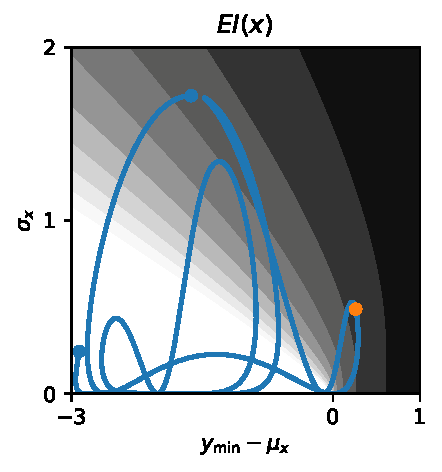
\includegraphics[width=0.8\textwidth]{Pictures/expected_improvement_illustration.pdf}
\end{figure}

In the following deveration
we assume the predictive distribution can be approxiamted by a normal distribution dependent on
the point of interest $x$ and the data $\mathcal{D}$ (note for the GP
it is in fact not an approximation), 
$$p(y|x,\mathcal{D}) \approx \mathcal{N}(y|\mu(x,\mathcal{D}), \sigma^2(x,\mathcal{D}))$$ where we
will change to a less clumpsy notation $\mathcal{N}(y|\mu_x,
\sigma^2_x):=\mathcal{N}(y|\mu(x,\mathcal{D}), \sigma^2(x,\mathcal{D}))$. This is completely fine
since we $x$ is fixed (and $\mathcal{D}$ is fixed) when evaluating the expected improvement in a point
$x$. %  $\sigma_x := \sigma^2(x,\mathcal{D})$ and $\mu_x := \mu(x,\mathcal{D})$
%as evaluated functions, i.e. numbers. 
Furthermore, the density of
a standard normal distribution is denoted $\phi(\cdot):=\mathcal{N}(\cdot | 0,1)$, and the cumlative
density function (CDF) of a standard normal distribution is denoted, $\Phi(\cdot) :=
\int_{-\infty}^{\cdot} \phi(\epsilon)d\epsilon$. We will now see that the normal approximation
of the predictive distribution yiels closed form solution to the expected improvement function, 

\begin{align*}
    E_{p(y|x,\mathcal{D})}[\max(0,y_{\min}-y)] &= \int \max(0,y_{\min}-y) p(y|x,\mathcal{D}) dy\\
    &\approx \int \max(0,y_{\min}-y) \mathcal{N}(y|\mu_x, \sigma_x^2) dy\\
    &= \int_{-\infty}^{y_{\min}} (y_{\min}-y) \frac{1}{\sigma_x}\phi\left(\frac{y-\mu_x}{\sigma_x}\right) dy\\
    &= \int_{-\infty}^{\frac{y_{\min}-\mu_x}{\sigma_x}} (y_{\min}-\mu_x-\sigma_x\epsilon) \frac{1}{\sigma_x}\phi\left(\epsilon\right) \sigma_x d\epsilon\\
    &= \int_{-\infty}^u \sigma_x \cdot (u-\epsilon) \phi(\epsilon) d\epsilon\\
    &=  \sigma_x \cdot \left( u\cdot \int_{-\infty}^u \phi(\epsilon) d\epsilon +\int_{-\infty}^u (-\epsilon)  \phi(\epsilon) d\epsilon \right) \\
    &= \sigma_x [u\Phi(u)+ \phi(u)]
\end{align*}

where $u:=\frac{y_{\min}-\mu_x}{\sigma_x}$. To understand the identity $\phi(u) = \int_{-\infty}^u
(-\epsilon)  \phi(\epsilon) d\epsilon$ used in the last equality, we first see that the antiderivative
is $\phi(\epsilon) = \frac{1}{\sqrt{2\pi}} \exp(\frac{-\epsilon^2}{2})$,
\begin{align*}
    \frac{d}{d \epsilon} \phi(\epsilon) &=  \frac{1}{\sqrt{2\pi}}\frac{d}{d \epsilon} \exp(\frac{-\epsilon^2}{2})\\
    &=  \frac{1}{\sqrt{2\pi}}\exp(\frac{-\epsilon^2}{2})(-\epsilon)\\
    &= -\epsilon \phi(\epsilon)
\end{align*}
and evaluating the rieman integral is equivalent to evaluate the antiderivative in its boundaries, giving the 
solution, 
$$\int_{-\infty}^u
(-\epsilon)  \phi(\epsilon) d\epsilon = \left[\phi(\epsilon)\right]_{-\infty}^u = \phi(u)-0 = \phi(u)$$ 

We can also explicily write the expected improvement as, 
$$EI(x) = (y_{\min}-\mu_x)\Phi\left(\frac{y_{\min}-\mu_x}{\sigma_x}\right)+ \sigma_x
\phi\left(\frac{y_{\min}-\mu_x}{\sigma_x}\right)]$$
where the first part can be interpretted as exploitation (favouring points with a large improvement $I(x) := (y_{\min}-\mu_x)$)
and the second part can be seen a exploitation (favouring points with high uncertainty.)
taking the derivative with respect to $I(x) := (y_{\min}-\mu_x)$ and $\sigma_x$, we see that expected improvement is 
is increasing if the improvement grows or if the variance $\sigma_x$ grows, i.e
$$\frac{\partial EI(x)}{\partial I(x)} = \Phi\left(\frac{y_{\min}-\mu_x}{\sigma_x}\right) > 0, \hspace*{0.5cm} 
\frac{\partial EI(x)}{\partial \sigma_x} = \phi\left(\frac{y_{\min}-\mu_x}{\sigma_x}\right) >0$$ 
<obs mistake in the book!!!?>





\begin{align*}
    \mathbb{E}_{y_*|\textbf{x}_*,D_n}[\max(0,y_{\min}-y_*)] &= ??\\
    \mathbb{E}[\min(0,y_{\min}-y_*)|\textbf{x}_*,D_n] &= \int_{-\infty}^\infty \min(0,y_{\min}-y_*) p(y_*|\textbf{x}_*,D_n) dy_*\\
    &= \int_{-\infty}^{y_{\min}} (y_{\min}-y_*) p(y_*|\textbf{x}_*,D_n) dy_*\\
    &\approx \frac{1}{N} \sum_{\theta \in \Omega } [y_{\min}-f_\theta(x)]
\end{align*}

where $\Omega = \{\theta|f_{\theta}(x)< y_{\min}\}$

%\section{uncertainties}
%Alatoric vs epistemic uncertainties 

\subsection{Entropy search}
We then discuss the knowledge
gradient (Section 4.2), entropy search and predictive entropy search (Section 4.3) acquisition functions.
These alternate acquisition functions are most useful in exotic problems where an assumption made by
expected improvement, that the primary benefit of sampling occurs through an improvement at the point
sampled, is no longer true.


The entropy search (ES) (Hennig and Schuler, 2012) acquisition function values the information we have
about the location of the global maximum according to its differential entropy

ES seeks the point to evaluate that causes the largest decrease in differential entropy

(Recall from, e.g., Cover and Thomas (2012),
that the differential entropy of a continuous probability distribution p(x) is R
p(x) log(p(x)) dx, and that
smaller differential entropy indicates less uncertainty.)

Predictive entropy search (PES) (Hern´andezLobato et al., 2014) seeks the same point, but uses a reformulation of the entropy reduction objective
based on mutual information. Exact calculations of PES and ES would give equivalent acquisition functions, but exact calculation is not typically possible, and so the difference in computational techniques
used to approximate the PES and ES acquisition functions creates practical differences in the sampling
decisions that result from the two approaches. We first discuss ES and then PES.

Let x  be the global optimum of f. The posterior distribution on f at time n induces a probability
distribution for x
. Indeed, if the domain A were finite, then we could represent f over its domain by a
vector (f(x) : x ∈ A), and x
would correspond to the largest element in this vector. The distribution of
this vector under the time-n posterior distribution would be multivariate normal, and this multivariate
normal distribution would imply the distribution of x

. When A is continuous, the same ideas apply,
where x

is a random variable whose distribution is implied by the Gaussian process posterior on f



\section{surrogate model}
As mentioned in the previous sections, the first of two repeated steps in Bayesian optimization
is to create a good Bayesian regression model. %why not non bayesian regression? 
i.e. finding the probility of prediction for a arbitrary point $x$ given datapoints 
$\mathcal{D} = \{x_1, y_1, \dots, x_n, y_n\}$, 
 $$p(y|x,\mathcal{D})$$

The surrogate model of choise in Bayesian optimization is a Gaussian Process, and Bayesian Neural Network.
These are discriminative models, however, another approach, which we focus on in this project, is
to model $y$ and $x$ jointly in a so-called generative model.



\subsection{Discriminative model as surrogate model}
When talking about a probabilistic surrogate model we are always implicit talking about a
discriminative model: A model of the conditional distribution of the observation, $y$, 
conditional on $x$, i.e., 
$$p(y|x)$$
we also refer to this as the predictive distribution. Gaussian processes and Bayesian neural networks
are both discriminative models. There is no distribution over the input $x$, it is just given. 
This is indeed sufficient for a surrogate model, where we are interested in the predictive distribution. 

\subsection{Using a generative model as surrogate model}

Given a generative model over $x$ and $y$ paramitised with $\theta$, we are dealing with the joint distribution
$$p(x,y|\theta)$$
and we are interested in the condtional distribution of y given x, 
$$p(y|x, \theta_{y|x})$$
where we have put subscript on $\theta$ in order to jump up a level of abstraction since, 
in fact there is just a mapping between them $\theta_{y|x} := g(\theta, y, x)$ 

% $$\alpha p(y|x) + (1-\alpha) \mathcal{N}(0,1)$$

% so what should $\alpha$ be? Here we can find inspiration from a Poission point process. 


\begin{align*}
    p(y|x, \mathcal{D}) &= \int p(y|x,\theta_{y|x})p(\theta_{y|x}|\mathcal{D}) d\theta_{y|x}  \\
    &=  p(y|x,\hat \theta_{y|x})
\end{align*}
Where the last equation holds as we assume that $p(\theta_{y|x}|\mathcal{D})$ is a delta function
i.e. a point estimate with value $\hat \theta_{y|x}$. In the case of our Gaussian mixture model, 
we obtain a point estiamte from the EM algorithm for the variance $\Sigma_{y|k}$, mean value $\mu_{y|k}$ and proportion $\pi_{y|k}$
for each component $k = 1,2, \dots, K$
$$\hat \theta_{y|x} = (\hat\Sigma_{y|k}, \hat\mu_{y|k}, \hat\pi_{y|k})_{k=1}^K$$

However, we are not satisfied with the variance estimate for the regression, as it is way too small for areas with
no observed data. It is therefore necessary to manipulate the variance estimate accoring to that observation. 
We multiply the variance obtained using expectation-maximization on the joint distribution with the 
inverse of the probability of the data $x$, and control that the scaling factor is not going wild!

$$\hat\Sigma_{y|k} =\Sigma_{y|k}^{GMM} \frac{1}{\max(p(x), 0.01)}$$

In a way, this is manipulation in a Bayesian spirit, as we let prior and subjective knowledge influence the
variance prediction. 
\subsection{Inclusion of prior distribution}
The new conditional distribution is essentially a mixture between the old conditional and the prior distribution, 
$$\hat p(y|x) = \alpha_x p(y|x) + (1-\alpha_x)p_{prior}(y)$$
where we choose $\alpha_x := \frac{S(x)}{S(x)+1}$. A convex combination of distributions is a distribution, 
since 
\begin{align*}
    \int_y \hat p(y|x) dy &= \int_y \left[ \alpha_x p(y|x) + (1-\alpha_x)p_{prior}(y) \right] dy\\
     &= \alpha_x \int_y p(y|x)dy +(1-\alpha_x) \int_y p_{prior}(y)dy \\
     &= \alpha_x + (1-\alpha_x) = 1
\end{align*}
    
\subsection{Inclusion of prior distribution}
Since the prior predictive distribution and the predictive distribution both are assumed to be normal distributions, 
it is possible to simply let the parameters of the manipulated predictive distributions be a convex combination of the 
parameters. This will make the manipulation be more natural, and hopefully less coruptive. 
\begin{align*}
    \hat p (y|x) &=\mathcal{N}(y| \hat \mu, \hat\sigma^2)\\
    \hat \mu &= \alpha \cdot \mu_{y|x} + (1-\alpha) \cdot \mu_{prior}\\
    \hat \sigma^2 &= \alpha \cdot \sigma_{y|x}^2 + (1-\alpha) \cdot\sigma_{prior}^2
\end{align*}


\subsection{Inclusion of prior distribution}
The conditional distribution $p(y|x)$ obtained from using a Gaussian mixture model is without a prior, and
the predictive distribution yields a way too small uncertainty estimate in regions where there are no observations.
This is because the range of the Gaussian distribution continues throughout the entire space and even though the
joint distribution is very small in the region, the conditional distribution is normalized using the (very small) $p(x)$.
We, therefore, want to introduce a prior, which can rule over the conditional in regions where the probability is too
small. The first approach is simply to define a new conditional distribution, 
\begin{align}\label{manipulated_pred_dist}
    \hat p(y|x) &\propto S(x) \cdot p(y|x) + p_{prior}(y)
\end{align}
where the scaling function can be interpreted as the probability of the input $x$ is in the region
ball $x \in B_{\frac{1}{2}\Delta}(x)$, and the probability density is not just $p(x)$ but the
probability of the average mixture component, which is $K\cdot p(x)$, assuming the mixture is
dominated be a single component at the position $x$. We define the scaling as 
$$S(x):= K\cdot p(x)\cdot \Delta$$
% $p_K(x)$ is the marginal density of an average mixture component, i.e. 
% $$p(x) = \sum_{k=1}^K \gamma_k p_k(x) \implies p_K(x) = K \cdot p(x)$$
Next we need to normalize the manipulated predictive distribution in order to
make it a proper probability density, i.e., making sure it integrates to 1, 
$$\int S(x) \cdot p(y|x) + p_{prior}(y) dy =S(x)+1$$
so the we can easily update \eqref{manipulated_pred_dist} with an equality
sign by defining the manipulated predive distribution as, 
$$\hat p(y|x) = \frac{S(x) \cdot p(y|x) + p_{prior}(y)}{S(x)+1}.$$

In figure \ref{pred_dist_manipulation} the manipulated predictive 
distribution is illustrated under the influenced of different scalings. 
Note that if $S(x) = 0$ the manipulated distribution becomes the prior,
while in the limit $S(x) \rightarrow \infty$ the manipulated distribution
become the original predictive distribtuion, $\hat p(y|x) = p(y|x)$. 

\begin{figure}[H]
    \centering
    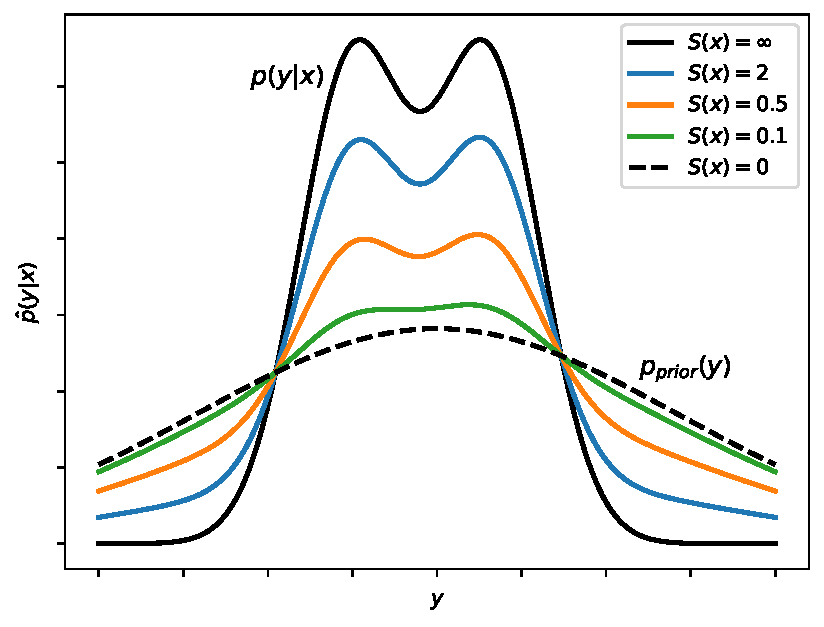
\includegraphics[width=0.45\textwidth]{Pictures/mixture_predictive_bayesian.pdf}
    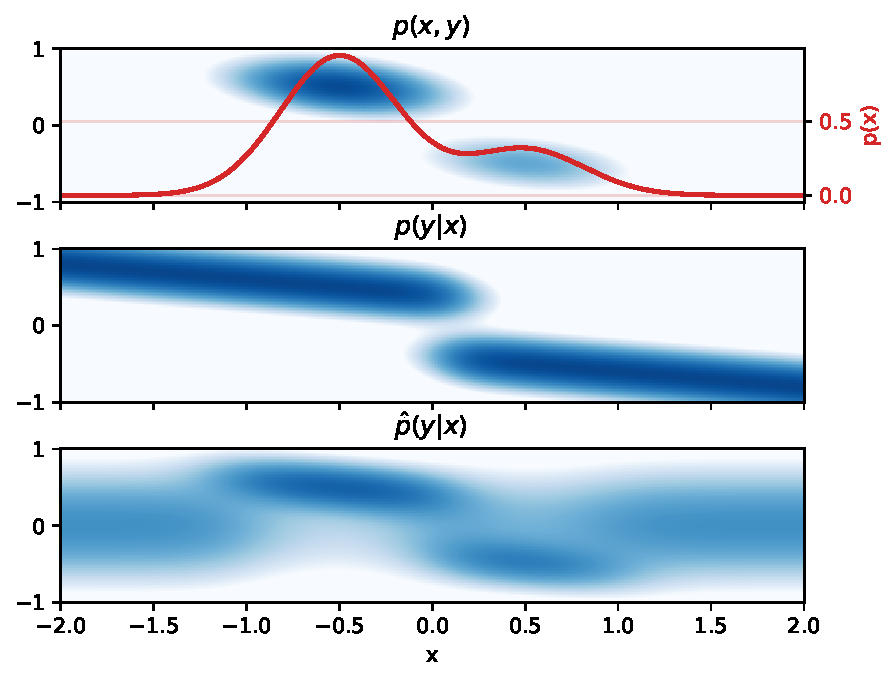
\includegraphics[width=0.45\textwidth]{Pictures/mixture_predictive_bayesian2D.pdf}
    \caption{Left: Illustration of how the preditive distribution is manipulated according
    the the scaling function $S(x) := p(x)\cdot N$. Right: Illustration of why it makes
    sense to manipulate the predictive distribution $p(y|x)$, if there is a small amount of input data
    at a region, then the predictive distribution should collapse into the uncertain prior}
    \label{pred_dist_manipulation}
\end{figure}

\subsubsection{Manipulated predictive mean}
What is the mean prediction of the manipulated predictive distribution?
\begin{align*}
    E_{p_{bayes}(y|x)}[y] &= \int y \cdot \frac{f(n,p(x)) \cdot p(y|x) + \lambda p_{prior}(y)}{Z} dy\\
    &= \left(p(x)\cdot N \cdot E_{p(y|x)}[y] + \lambda \cdot E_{p_{prior}(y)}[y] \right) \frac{1}{Z}\\
    &= \frac{p(x)\cdot N\cdot E_{p(y|x)}[y]}{p(x)\cdot N+\lambda}
\end{align*}

\subsubsection{Manipulated predictive variance}
What is the variance of the manipulated predictive distribution
We first calculate the second moment, 
\begin{align*}
    E_{p_{bayes}(y|x)}[y^2] &= \int y^2 \cdot \frac{p(x)\cdot N \cdot p(y|x) + \lambda p_{prior}(y)}{Z} dy\\
    &= (p(x)\cdot N\cdot E_{p(y|x)}[y^2] + \lambda E_{p_{prior}(y)}[y^2] ) \frac{1}{Z}\\
    &= \frac{p(x)\cdot N \cdot(Var_{p(y|x)}[y]+E_{p(y|x)}[y]^2) + \lambda Var_{p_{prior}(y)}[y]}{p(x)\cdot N+\lambda}
\end{align*}

So the variance is calculated as, 
$$V_{p_{bayes}(y|x)}[y] = E_{p_{bayes}(y|x)}[y^2] - E_{p(x,y)}[y]^2$$

\subsubsection*{implementation}
It is not necessary to calculate the conditional distribution, since, using Bayes rule
$$p(y|x) = \frac{p(x,y)}{p(x)}$$
so gives
$$p_{bayes}(y|x) = \frac{p(x)\cdot N \cdot p(y|x) + \lambda p_{prior}(y)}{Z} = \frac{N \cdot p(x,y) + \lambda p_{prior}(y)}{Z}$$

$$E_{p(x,y)}[y] = \int_y \int_x yp(x,y) dx dy = \int_y y p(y) dy = E_{p(y)}[y]$$


\section{Inference of surrogate models}
Inference is the process of computing answers to queries about a probabilistic model after observing data. 
In Bayesian regression, the
query is the predictive distribution, $p(y|x,\mathcal{D})$, as we are interested in the distribution of $y$ given $x$ 
and already observed data, $\mathcal{D}$. 
This often indirectly create the posterior query, $p(\theta|\mathcal{D})$, the probability of model parameters $\theta$ given data
$\mathcal{D}$. Lastly it is also inference, when we train 
a Gaussian mixture model or SPN using the expectation-maximization algorithm (EM), since we are iteratively answering the query
$E_{p(z|\theta^{(k)})}[z|\theta]$.

%\subsection{Exact and approximate inference}
We distinguish between two different ways of inference, exact and approximate inference.
It is \textit{exact inference} when a probabilistic query is calculated exact. It is possible to calculate exact inference on 
the predictive distribution for the Gaussian mixture model, Sum product network, and Gaussian processes. Models which allow 
for exact inference have a powerful advantage over the models with approximate inference since we can guarantee
 the answers to the queries are
correct, however, they are usually also less expressive. It is possible to
make exact inference of SPN, Gaussian Process, and Gaussian Mixture Regression. 
% \begin{itemize}
%     \item SPN
%     \item Gaussian Process
%     \item Gaussian Mixture Regression
% \end{itemize}

When it is not possible to answer a probabilistic query exact, we can approximate the
answer using \textit{approximate inference}. When dealing with complicated and expressive statistical models, exact inference is often
intractable and we need to use approximate inference. Approximate inference 
is a broad category of methods, which includes 
variational inference, Laplace approximation, and Markov chain Monte Carlo (MCMC).
The two Bayesian Neural networks we deal with in this project Bohamiann and Numpyro BNN are
similar regression models, but are infered using two different versions of the MCMC 
method, Hamiltonian Monte Carlo. As it will be revealed later (see result section) 
approximate inference might indeed be flawed and inexact. 
%When dealing with complicated and expressive statistical models, exact inference is often
%intractable and we need to use approximate inference, which might indeed be flawed and 
%inexact. 
% \begin{itemize}
%     \item Bohamiann (Adaptive stochastic MCMC)
%     \item Numpyro Bayesian Neural Network (NUTS)
% \end{itemize}

\begin{table}[H]
    \centering
    \begin{tabular}{l|l|l}
    %\rowcolor[HTML]{C0C0C0} 
    \textbf{Model} & \textbf{Predictive inference} &   \textbf{Learning} \\ \hline
    GP          & Exact $O(n^3)$  & Emperical Bayes\\
    SPN             & Exact $O(E)$ &  EM $O(E)$\\
    Gaussian Mixture Regression & Exact $O(K)$ & EM  \\
    Bohamiann                             & Adaptive stochatic HMC & \\
    Numpyro BNN                           & No U-Turn Sampler & 
    \end{tabular}
    \caption{Overview of inference methods applied on the statistical models 
            used in this project. $E$ is the number of edges in the SPN. $n$ is the number of datapoints. 
            $K \leq n$ is the number of mixture comonents. We will soon learn that for an
            SPN the number of mixture compenets is exponential larger than number of edges
            i.e. $E << K$. In theory MCMC methods samples 
            from true the posterior distribution, and do not need any fitting/learning. 
            }
\end{table}